\newpage
\noindent
\vspace*{-2.0cm}
\section*{\sectionformat Nome da Receita}
\addcontentsline{toc}{section}{Nome da Receita}
\vspace*{-0.1cm}
\begin{aemulticol}[width=0.495\textwidth,height=0.545\textheight]
	\begin{tabu} to 0.5\linewidth {X[l]X[r]}
	   \textit{Serve $3$ pessoas} & \textit{$430$ kcal}
	\end{tabu}\\
	\rule[0.5ex]{0.5\linewidth}{1pt}
	
	\vspace*{-0.3cm}
	\subsection*{\subsectionformat Ingredientes}
	\vspace*{-0.15cm}
	\begin{tabu} to 0.5\linewidth {X[l]X[l]}
	   $\bullet$ ingrediente com nome muito grande grande demais mesmo que cai pra outra linha & $\bullet$ ingrediente\\
	   $\bullet$ ingrediente & $\bullet$ ingrediente\\
	   $\bullet$ ingrediente & $\bullet$ ingrediente\\
	   $\bullet$ ingrediente & $\bullet$ ingrediente\\
	   $\bullet$ ingrediente & $\bullet$ ingrediente
	\end{tabu}

	\vspace*{-0.15cm}
	\subsection*{\subsectionformat Modo de Preparo}
	\vspace*{-0.15cm}
	$1.$  Passo 1\\
	$2.$  Passo 2\\
	$3.$  Passo 3\\
	$4.$  Passo 4\\
	$5.$  Passo 5\\
	$6.$  Passo 6\\
	$7.$  Passo 7\\
	$8.$  Passo 8\\
	$9.$  Passo 9\\
	$10.$ Passo 10\\
	$11.$ Passo 11\\
	$12.$ Passo 12\\
	$13.$ Passo 13\\
	$14.$ Passo 14\\
	$15.$ Passo 15\\
	$16.$ Passo 16\\
	$17.$ Passo 17\\
	$18.$ Passo 18\\
	$13.$ Passo 13\\
	$14.$ Passo 14\\
	$16.$ Passo 16\\
	$17.$ Passo 17\\
	$18.$ Passo 18\\
	$13.$ Passo 13\\
	$14.$ Passo 14\\
	$16.$ Passo 16\\
	$17.$ Passo 17\\
	$18.$ Passo 18\\
	$13.$ Passo 13\\
	$14.$ Passo 14\\
	$15.$ Passo 15\\
	$16.$ Passo 16\\
	$17.$ Passo 17\\
	$18.$ Passo 18\\
	$19.$ Passo 19	

	\vspace*{-0.15cm}
	\subsection*{\subsectionformat Dicas}
	\vspace*{-0.15cm}
	
	$\bullet$ Dica 1\\
	$\bullet$ Dica 2\\
	$\bullet$ Dica 3
	
	\vspace*{-0.15cm}
	\subsection*{\subsectionformat História}
	\vspace*{-0.15cm}
	\textit{Essa receita foi criada para testar o layout do livro e infelizmente, provavelmente nunca será feita. Coitada da receita.}
\end{aemulticol}
\begin{tikzpicture}[remember picture, overlay]
\node[anchor = south, inner sep = 0pt, outer sep = 0pt] at (current page.south) 
{
	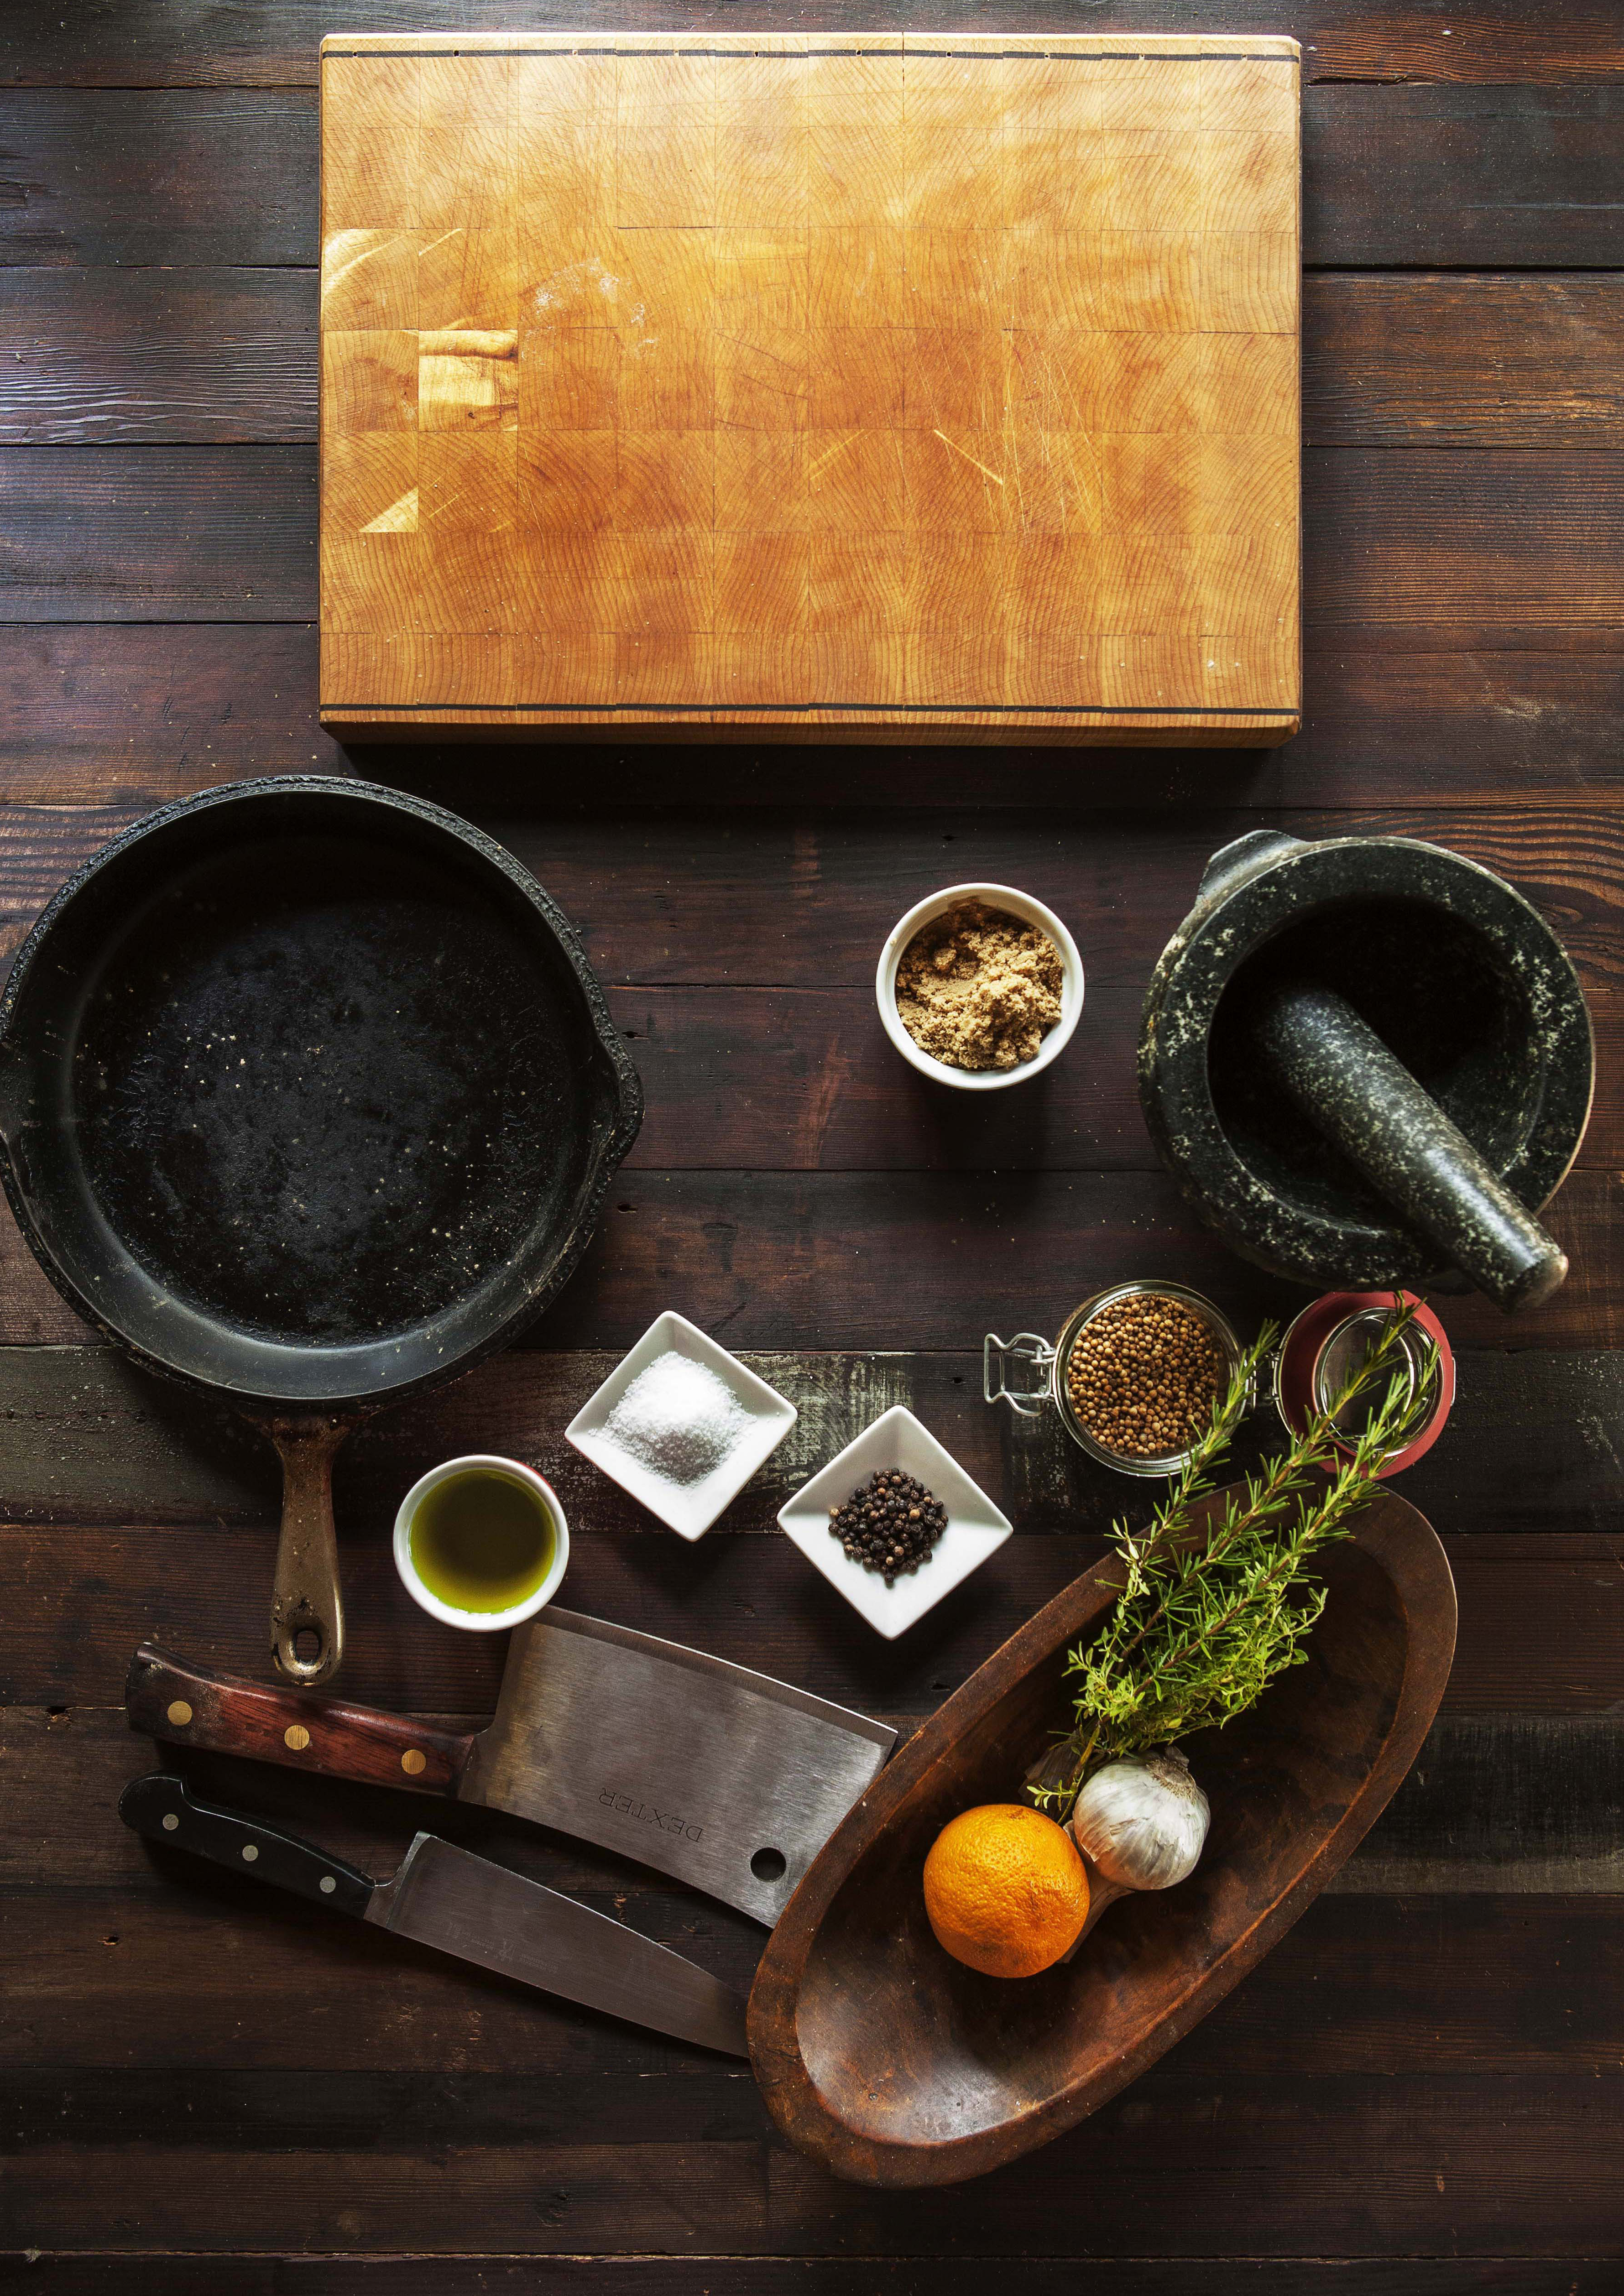
\includegraphics[width=\paperwidth, height=0.45\paperheight]{cover.jpg}
};
\end{tikzpicture}